\chapter{Reflexions sobre la informació en la multiresolució}
\label{sec:multiresolucio:teoriainformacio}



En aquest capítol reflexionem sobre el problema de la qualitat en la
multiresolució de sèries temporals, és a dir sobre el problema
d'identificar la informació que selecciona un esquema de
multiresolució i per tant, alhora, d'observar quina informació no
queda emmagatzemada i es perd.  Contextualitzem aquest problema en
l'aplicació de la teoria de la informació per a l'esquema de
multiresolució.

En aquest context, els \gls{SGSTM} són un sistemes que emmagatzemen
dades comprimides amb pèrdua d'una certa part de la informació
original. Aleshores, les consultes que es resolen a partir d'un
\gls{SGSTM} són consultes aproximades a la informació total original,
llevat que mitjançant una anàlisi determinem que poden oferir
consultes exactes. A continuació reflexionem sobre com analitzar
l'error de les consultes de multiresolució respecte a la informació
original:
\begin{itemize}
\item Primer, descrivim de forma molt genèrica la teoria de la
  informació, la qual està relacionada amb la quantificació de la
  informació.
\item Segon, definim el problema de calcular l'error en la multiresolució.
\item Tercer, mostrem exemples d'anàlisi de la informació per alguns
  esquemes de multiresolució.
\end{itemize}






\section{Quantificació de la informació}

En altres àmbits, la teoria de la informació (\emph{information
  theory}) és la teoria de referència per a formalitzar la
quantificació de la informació. Aquest també és el cas de la
compressió de dades, un àmbit proper als \gls{SGSTM} en aquest context
d'informació.  Per al cas particular de compressió amb pèrdua s'aplica
un subconjunt de la teoria anomenat teoria de la taxa de
bit-distorsió %optimot: rate-distortion relationship
(\emph{rate–distortion theory}); la qual modela la percepció de la
distorsió i valora l'estètica dels resultats.


Per a quantificar la informació d'unes dades s'utilitza l'entropia, la
qual mesura la incertesa que hi ha en unes dades particulars. Així,
com més entropia més incertesa, a causa que les dades són més
aleatòries, i com menys entropia més facilitat de predir-les a causa
que són més redundants. Si l'entropia és zero aleshores les dades són
totalment predictibles; és a dir donat un valor es coneix exactament
quin és el següent.




La compressió redueix la mida original de les dades. En el cas de la
compressió sense pèrdua es conserva la informació però s'augmenta
l'entropia, ja que s'eliminen les dades redundants. En el cas de la
compressió amb pèrdua es descarta informació que es considera no
essencial. Un exemple de compressió amb pèrdua és eliminar detalls
d'una imatge que l'ull humà no pot apreciar. A més, la compressió amb
pèrdua també es pot utilitzar per a transformar les dades a un altre
domini on es percebi millor la informació, la qual cosa es coneix amb
el nom de codificació perceptiva (\emph{perceptual encoding}). Un
exemple de codificació perceptiva és transformar els sons al domini
freqüencial per a operacions d'equalització.



Els mètodes de compressió amb pèrdua se solen usar per a compressió de
multimèdia. L'objectiu és aconseguir menys volum de dades però que
conservin la mateixa percepció que les originals, o fins i tot amb una
pèrdua de qualitat perceptible mentre compleixi amb els requisits de
l'aplicació que se li vol donar. Així doncs, la compressió de
multimèdia sovint requereix valorar la percepció humana, per tal de
valorar la qualitat de percepció humana s'utilitzen testos subjectius
en què un humà ha d'intentar distingir entre multimèdia original i
multimèdia comprimit.
%  com per exemple el test
% ABX\todo{ref}.  %http://en.wikipedia.org/wiki/ABX_test
%http://web.archive.org/web/20070813001013/http://www.pcabx.com/


%  Lossy methods are most often used for compressing sound, images or videos. This is because these types of data are intended for human interpretation where the mind can easily "fill in the blanks" or see past very minor errors or inconsistencies – ideally lossy compression is transparent (imperceptible), which can be verified via an ABX test. http://en.wikipedia.org/wiki/ABX_test
% Flaws caused by lossy compression that are noticeable to the human eye or ear are known as compression artifacts.




% \todo{information algebra}
% \url{https://en.wikipedia.org/wiki/Information_algebra}

% algebra of information, describing basic modes of information processing. Such an algebra involves several formalisms of computer science, which seem to be different on the surface: relational databases, multiple systems of formal logic or numerical problems of linear algebra. It 



% El procediment
% que se segueix és: comprimir, emmagatzemar, descomprimir i
% visualitzar.
% compressed data must be decompressed to use -> en els sgstm no? bé si vull veure tota la sèrie temporal sí que he de concatenar el que hi tinc i per tant es pot veure com una descompressió (al marge que hi pot haver una compressió/descompressió en els agregadors usats, per exemple si és un so emmatgatzemar la freqüència i després s'haurà de descomprimir a amplitud al llarg del temps).
% The design of data compression schemes involves trade-offs among various factors, including the degree of compression, the amount of distortion introduced (e.g., when using lossy data compression), and the computational resources required to compress and uncompress the data.
% * No hi ha descompressió. Els algoritmes de compressió amb pèrdua normalment van associats amb les tècniques de compressió/descompressió; és a dir que les dades s'emmagatzemen amb estructures intermitges, que ocupen menys mida, i que cal descomprimir per recuperar-les. En els cas dels SGSTM les dades s'emmagatzemen com a subsèries temporals en els discs i per tant a l'hora de recuperar-les ja són sèries temporals, com a molt potser fa falta concatenar-les per a obtenir tota la sèrie temporal.



% The main drawback of lossy compression techniques is that they
% rely on specific patterns for providing a good approximation of the given time series.
% This is the main reason why lossy compression has been rarely applied to network
% monitoring contexts, where the patterns of time series can drastically change due to
% anomalous events or to transient networking issues.

%http://www.data-compression.com/theory.shtml


\section{Error en la informació de la multiresolució}

El model dels \gls{SGSTM} es basa en una compressió amb pèrdua, és a
dir descartar dades i emmagatzemar només aquella informació que es
consideri necessària o suficient. Així doncs, cal quantificar quin
error hi ha entre la informació emmagatzemada i la informació que
contenen les dades originals.


El problema genèric de la informació en la multiresolució és el següent.
\begin{definition}[Error en la informació de la multiresolució]
  \label{def:informacio:error}
  Sigui una sèrie temporal $S$ i una sèrie temporal multiresolució $M$
  resultant de l'emmagatzematge i consolidació de $S$. De la sèrie
  temporal multiresolució es pot consultar la sèrie temporal total
  $S'=\glssymbol{not:sgstm:serietotal}(M)$ o bé de forma equivalent,
  com s'ha descrit en \textref{cap:funciomultiresolucio},
  $S'=\glssymbol{not:sgstm:multiresolucio}(S,\glssymbol{not:esquemaM})$
  on $\glssymbol{not:esquemaM}$ és l'esquema de $M$.  S'executa una
  operació de consulta, $o$, sobre la sèrie temporal original,
  $r_1=o(S)$, i la mateixa operació sobre la sèrie temporal de la
  multiresolució, $r_2=o(S')$. Es pot avaluar l'error de
  multiresolució $\epsilon=d(r_1,r_2)$ on $d$ és una funció que permet
  avaluar la distància entre els dos resultats i per tant considerem
  $\epsilon\geq 0$.
\end{definition}


Cal aclarir que es podria avaluar $d(S,S')$ com un problema
d'aproximació al senyal original. Aquest és un problema ben resolt en
altres models, com per exemple \textcite{last01,ogras06}, però no és
el problema que es vol resoldre en els \gls{SGSTM}.  L'objectiu dels
\gls{SGSTM} és comprimir les dades i seleccionar una determinada
informació, per tant és un problema de compressió amb pèrdua.  Així
doncs, ens interessa avaluar l'error de la multiresolució en aquest
context, en què les consultes als \gls{SGSTM} ($r_2$) haurien de
retornar resultats similars que si es fessin a les dades originals
($r_1$), sense que sigui necessari que $S$ i $S'$ es corresponguin.




Per a avaluar la distància $d(r_1,r_2)$, si els resultats d'ambdues
consultes són sèries temporals, es pot utilitzar per exemple mínims
quadrats com fa \textcite{last01}.  Ara bé, en la informació de la
multiresolució cal pensar també amb consultes qualitatives. Per
exemple una consulta podria ser $o=$`Creix la sèrie temporal?'
Aleshores no hi hauria error $\epsilon=d(r_1,r_2)$ quan la resposta
fos la mateixa per als dos casos, $r_1$ i $r_2$, i hi hauria error
quan les respostes diferissin.



Tot i que hem proposat d'aplicar la mateixa operació $o$ a la sèrie
temporal original $r_1=o(S)$ i a la sèrie temporal de la
multiresolució $r_2=o(S')$, pot ser que l'operació hagi de ser
diferent per a obtenir el mateix resultat. És a dir $r_1=o(S)$ però
$r_2=o'(S')$ on $o'$ és l'operació equivalent a $o$ que s'ha d'aplicar
després de la multiresolució.  Per exemple, una operació $o$ podria
ser el càlcul de la multiresolució,
$r_1=\glssymbol{not:sgstm:multiresolucio}(S,\glssymbol{not:esquemaM})$,
aleshores l'operació $o'$ equivalent és la identitat perquè el
\gls{SGSTM} ja ha calculat la multiresolució, $r_2=S'$. Aquest
exemple, de fet, és el cas que hem formulat a la
\autoref{sec:multiresolucio:funcio}, on hem descrit l'equivalència
entre la sèrie temporal total d'un \gls{SGSTM} i la funció
\glssymbol{not:sgstm:multiresolucio} d'una sèrie temporal; per tant
l'error $\epsilon =d(r_1,r_2)$ seria nul.



Així doncs, l'error en la informació de la multiresolució permet
quantificar la pèrdua d'informació dels \gls{SGSTM}. Un cop
quantificat l'error per a un determinat esquema de multiresolució es
pot saber per a quines consultes serà apropiat aquell esquema i per a
quines no. Per a quantificar aquest error es poden preveure diversos
contextos:
\begin{itemize}
\item Hi ha consultes que es poden resoldre a la perfecció, és a dir
  sense error. Per exemple és el cas descrit on l'operació que es vol
  fer a una sèrie temporal és precisament la consulta de
  multiresolució.
  %altres exemples, per exemple en el cas de comptadors per a consultar totals

\item Es pot calcular l'error mesurant la diferència entre la mateixa
  consulta aplicada a les dades originals que a les dades
  emmagatzemades en el \gls{SGSTM}.

\item Es pot avaluar subjectivament l'error mitjançant la
  visualització de les dades. És a dir, de manera semblant a la
  compressió amb pèrdua de multimèdia, l'usuari valora subjectivament
  si visualitza la mateixa informació en les dades originals com en
  les dades comprimides amb multiresolució. Per exemple, un dels
  criteris que recomana RRDtool per a establir un esquema de
  multiresolució és tenir en compte l'amplada de la pantalla on es
  visualitzen els resultats: no cal treballar amb una sèrie temporal
  amb molta resolució si no és possible observar-la \parencite[Rates,
  normalizing and consolidating]{vandenbogaerdt} .
  % RRDtool expliquen un criteri que és definir les k dels discs inferior a l'amplada en píxels de la pantalla. Aquest és un criteri basat en una consulta per a fer visualització immediatament. Llavors no té sentit tenir més nombre de dades que les que es poden visualitzar.  Per exemple si capturem dades cada 5 minuts al llarg d'un any obtenim 43800 punts; si no disposem d'un monitor amb aquest nombre de píxels d'amplada no els podrem percebre.
  %Això potser també té relació amb el camp de gràfics 3D, on la multiresolució s'aplica per a no treballar amb objectes que només seran percebuts com un píxel?

\end{itemize}






\section{Exemples d'anàlisi de la informació}


La \autoref{def:informacio:error} descriu el problema d'informació en
la multiresolució de forma genèrica i abstracta. Així, en cada context
d'aplicació de la multiresolució cal interpretar-ne el significat i
particularitzar-ne un mètode d'anàlisi adequat.  A tal efecte, a
continuació proposem alguns exemples que mostren casos particulars
d'anàlisi de la selecció o pèrdua d'informació que hi ha en un
\gls{SGSTM}.


Per a simplificar els exemples, proposem esquemes de multiresolució amb
només una resolució i amb funcions d'agregacions d'atributs que
seleccionen intervals independents de mesures. Per tal de referir-nos
amb comoditat als càlculs de les funcions d'agregació d'atributs,
anomenem les mesures i els valors amb els quals operen mitjançant la
notació següent.



\begin{definition}[Notació de les mesures i els valors amb els quals operen
  les funcions d'agregació d'atributs]
  \label{def:informacio:notaciovalors}
  Sigui $S=\{m_0,\dotsc,m_k\}$ una sèrie temporal, on recordem que les
  mesures tenen la forma $m=(t,v)$, i $\glssymbol{not:esquemaM}= \{
  (\delta, \glssymbol{not:sgstm:f} , \tau, \glssymbol{not:sgstm:k})
  \}$ un esquema de multiresolució amb una sola subsèrie
  resolució. Assumim $ \glssymbol{not:sgstm:k}=\infty$ per tal de
  negligir-ne l'efecte i $\tau=T(\min S)$. Obtenim la sèrie temporal
  resultant de la funció de multiresolució
  $S'=\glssymbol{not:sgstm:multiresolucio}(S,\glssymbol{not:esquemaM})$
  (\seeref{def:multiresolucio:plecmu}).  Així, aquesta sèrie temporal
  resultant conté mesures calculades a partir de l'agregació de $S$ en
  els intervals definits per $\tau$ i $\delta$ i té la forma
  \begin{align*}
    S'=  \{ & \glssymbol{not:sgstm:f}(S,\tau,\delta), \\
    & \glssymbol{not:sgstm:f}(S,\tau+\delta,\delta),\\
    &\dotsc, \\
    & \glssymbol{not:sgstm:f}(S,\tau+(n-1)\delta,\delta)\}
  \end{align*}
  on $\tau+n\delta\geq T(\max S)$ i $n\in\glssymbol{not:N}$.


  La funció d'agregació d'atributs $\glssymbol{not:sgstm:f}$ realitza
  una operació sobre les mesures corresponents a l'interval de temps
  definit (\seeref{sec:model:agregador}).  Així per a l'agregació en
  el primer interval $[\tau,\tau+\delta]$ escriurem de forma genèrica
  que utilitza les mesures $m_0,\dotsc,m_{i_1}$ de la sèrie temporal
  original, $m_0,\dotsc,m_{i_1} \in S$ on $i_1$ pot ser qualsevol
  índex, i per tant escriurem els valors corresponent a aquestes
  mesures com $v_0,\dotsc,v_{i_1}$. De la mateixa manera, escriurem
  $m_{i_1+1},\dotsc,m_{i_2}$ i $v_{i_1+1},\dotsc,v_{i_2}$ per a
  l'agregació en el segon interval,
  $[\tau+\delta,\tau+2\delta]$, i així successivament
  fins al darrer interval en què notem les mesures amb $m_{i_n},
  \dotsc, m_k$ i els valors amb $v_{i_n}, \dotsc, v_k$.
%és a dir s'utilitzen les mesures de forma independent a cada interval, segons les opcions descrites a les famílies d'agregacions aquí simplifiquem i no introduïm els casos en què una mesura s'utilitza en més d'un interval, per exemple en el ZOHE hauríem de formular com s'escampa la informació en més d'un interval

  Aleshores, a partir de la notació dels valors, podem expressar la
  sèrie temporal resultant amb la forma
  \begin{align*}
    S'=\{& (\tau+\delta, f'(v_0,\dotsc,v_{i_1})),\\
    & (\tau+2\delta, f'(v_{i_1+1},\dotsc,v_{i_2})),\\
    & \dotsc,\\
    & ((\tau+n\delta ,f'(v_{i_M},\dotsc, v_k)) \}
  \end{align*}
  on $f'$ és l'operació corresponent de l'atribut que resumeix
  $f$. En els exemples següents assenyalarem quin $f'$ correspon a
  cada $f$ que utilitzem.
\end{definition}



L'anàlisi que formulem és una introducció a la reflexió sobre l'error
en la informació de la multiresolució. Així, de forma simple,
analitzem si hi ha error o si no n'hi ha, sense pretendre avaluar
quantificacions més complicades. A més, ho analitzem en base a
l'esquema de multiresolució que s'utilitzi, particularment de quines
funcions d'agregació d'atributs s'utilitzin i de com siguin les
consultes posteriors.



\subsection{Mateixa consulta i funció d'agregació d'atributs}
\label{ex:multiresolucio:f=op}


En aquest apartat es formulen exemples que reflexionen sobre l'error
de multiresolució que hi pot haver quan una consulta s'aplica a tota
la sèrie temporal i l'operació de consulta es correspon amb la mateixa
funció d'agregació d'atributs que s'ha utilitzat en l'esquema de
multiresolució.


% Sigui $S=\{m_0,\dotsc,m_k\}$ una sèrie temporal, on $m_k=(t_k,v_k)$, i
% $e= \{ (\delta_0, f_0, \tau_0, k_0) \}$ un esquema de multiresolució
% amb una sola subsèrie resolució, suposem $k_0=\infty$ per tal de
% negligir-ne l'efecte i $\tau_0=T(\min(S))$. Obtenim la sèrie temporal
% resultant d'aplicar la funció de multiresolució
% $S'=\glssymbol{not:sgstm:multiresolucio}(S,e)$.  Així, aquesta sèrie
% temporal resultant contindrà mesures calculades a partir de
% l'agregació de $S$ en els intervals definits per $\tau_0$ i $\delta_0$
% i tindrà la forma $S'=\{ f_0(S,[\tau_0,\tau_0+\delta_0],
% f_0(S,[\tau_0+\delta_0,\tau_0+2\delta_0]),\dotsc,
% f_0(S,[\tau_0+(M-1)\delta_0,\tau_0+M\delta_0])\}$ on
% $\tau_0+M\delta\geq T(\max(S))$ i $M\in\glssymbol{not:N}$. Si escrivim
% de forma genèrica $v_0,\dotsc,v_{i_1}$ els valors originals usats en
% l'agregació del primer interval $f_0(S,[\tau_0,\tau_0+\delta_0])$,
% $v_{i_1+1},\dotsc,v_{i_2}$ els del segon interval, etc. aleshores
% podem expressar $S'=\{ (\tau_0+\delta_0, f'(v_0,\dotsc,v_{i_1})),
% (\tau_0+2\delta_0, f'(v_{i_1+1},\dotsc,v_{i_2})), \dotsc,
% ((\tau_0+M\delta_0 ,f'(v_{i_M}, \dotsc, v_k)) \}$ on $f'$ és
% l'aplicació corresponent de l'atribut que resumeix $f_0$.


El context del problema és el següent. S'aplica un operador de
consulta $o$ a les dues sèries temporals, $r_1=o(S)$ i $r_2=o(S')$.
Aquest operador $o$ és el mateix càlcul que fa la funció d'agregació
d'atributs $f$ però aplicat a totes les mesures de la sèrie temporal
original, $o(S)=V(f(S,[-\infty,\infty]))$. Analitzem l'error de
multiresolució entre $r_1$ i $r_2$ segons tres funcions d'agregació
d'atributs:

  \begin{itemize}
  \item Màxim: $f=\glssymbol{not:sgstm:maxpd}$, el qual es correspon
    a aplicar l'operació d'agregació dels \glspl{SGST}
    $o=\glssymbol{not:sgst:maxv}$ (\seeref{def:sgstm:maxpd}) i per
    tant a calcular l'atribut $f'=\max$ dels valors (\seeref{def:sgst:maxv}).

    D'una banda $S=\{m_0,\dotsc,m_k\}$ i aleshores
    $r_1=o(S)=\glssymbol{not:sgst:maxv}(S) = \max(v_0,\dotsc,
    v_k)$. D'altra banda, aplicant la notació de la
    \textref{def:informacio:notaciovalors}, $S'=\{ (\tau+\delta,
    \max(v_0,\dotsc,v_{i_1})),
    (\tau+2\delta,\max(v_{i_1+1},\dotsc,v_{i_2})), \dotsc,
    (\tau+n\delta,\max(v_{i_n}, \dotsc, v_k)) \}$ i aleshores
    $r_2=o(S')= \max\big( \max(v_0,\dotsc,v_{i_1}),
    \max(v_{i_1+1},\dotsc,v_{i_2}), \dotsc, \max(v_{i_n}, \dotsc v_k)
    \big)$.

    Atès que $\max(v_0,\dotsc, v_k) = \max\big(
    \max(v_0,\dotsc,v_{i_1}), \max(v_{i_1+1},\dotsc,v_{i_2}), \dotsc,
    \max(v_{i_n}, \dotsc v_k) \big)$ perquè $\max$ és una funció
    associativa: $\max(a,b,c,d,e) = \max( \max(a,b), \max(c,d,e))$,
    podem concloure que en aquest cas $r_1=r_2$ i per tant
    $\epsilon=0$.


    En aquest exemple hem negligit els temps resultants de
    l'agregació. És a dir, $r_1$ és correspon amb una o més d'una
    mesura $m\in S: V(m)=r_1$ i de la mateixa manera $n\in S':
    V(n)=r_2$ on hem conclòs que $V(m)=V(n)$. Això no obstant,
    en general els temps d'aquestes mesures no es correspondran,
    $T(m)\neq T(n)$ perquè $f=\glssymbol{not:sgstm:maxpd}$
    resumeix els atributs de temps segons l'interval de consolidació i
    al marge del resum de la informació en els valors.



  \item Mitjana aritmètica: $f=\glssymbol{not:sgstm:mitjanapd}$, el
    qual es correspon a aplicar l'operació d'agregació dels
    \glspl{SGST} $o=\glssymbol{not:sgst:mitjanav}$
    (\seeref{def:sgstm:mitjanapd}) i per tant a calcular l'atribut
    $f'=\operatorname{mitjana}$ (aritmètica) dels valors
    (\seeref{def:sgst:mitjanav}).

    De manera similar al cas anterior, els resultats són
    $r_1=\operatorname{mitjana}(v_0,\dotsc, v_k)$ i
    $r_2=\operatorname{mitjana}\big(
    \operatorname{mitjana}(v_0,\dotsc,v_{i_1}),
    \operatorname{mitjana}(v_{i_1+1},\dotsc,v_{i_2}), \dotsc,
    \operatorname{mitjana}(v_{i_n}, \dotsc v_k) \big)$.  Però en
    aquest cas hem de concloure que $\epsilon\geq 0$ perquè
    la mitjana no és una funció associativa:
    $\operatorname{mitjana}(a,b,c,d,e) \neq \operatorname{mitjana}(
    \operatorname{mitjana}(a,b), \operatorname{mitjana}(c,d,e))$.
 


  \item Total: definim una funció d'agregació d'atributs
    $f=\operatorname{total}$ que, negligint l'atribut de temps,
    resumeix la sèrie temporal amb la suma dels valors:
    $\operatorname{total}(S,\tau,\delta)=m'$  i $V(m') =
    \sum\limits_{\forall m\in S(\tau,\tau+\delta]} V(m)$. Així doncs, es
    correspon a aplicar l'operació d'agregació dels \glspl{SGST}
    $o=\glssymbol{not:sgst:sumav}$ i per tant a calcular l'atribut
    $f'=\sum$ dels valors (\seeref{def:sgst:sumav}).

    Aquest cas és similar al del màxim, $r_1=\sum(v_0,\dotsc, v_k)$ i
    $r_2=\sum\big( \sum(v_0,\dotsc,v_{i_1}),
    \sum(v_{i_1+1},\dotsc,v_{i_2}), \dotsc, \sum(v_{i_n}, \dotsc v_k)
    \big)$, i $\epsilon=0$ perquè la suma és una funció
    associativa.
    

  \end{itemize}


\subsection{Mitjana d'una sèrie temporal regular}

  Seguint \textref{ex:multiresolucio:f=op}, podem estudiar en quins
  casos la mitjana aritmètica no té error. Com ja s'ha dit, la mitjana
  no és una funció associativa. Però sí que esdevé associativa quan
  s'associen el mateix nombre d'elements:
  $\operatorname{mitjana}(a,b,c,d,e,f) = \operatorname{mitjana}(
  \operatorname{mitjana}(a,b), \operatorname{mitjana}(c,d),
  \operatorname{mitjana}(e,f)) = \operatorname{mitjana}(
  \operatorname{mitjana}(a,b,c), \operatorname{mitjana}(d,e,f))$.

  Per tal que s'associïn el mateix nombre d'elements cal que per cada
  interval de consolidació de la sèrie temporal hi hagi el mateix
  nombre de mesures:
  $|S[\tau,\tau+\delta]|=|S[\tau+\delta,\tau+2\delta]|=\dotsb
  = |S[\tau+(n-1)\delta,\tau+n\delta]|$.  Aquest cas es
  compleix, per exemple, quan la sèrie temporal és regular amb període
  $p$ i el pas de consolidació de l'esquema multiresolució és múltiple
  de la regularitat de la sèrie temporal, $\delta = kp$ on
  $k\in\glssymbol{not:N}$, o bé quan la sèrie temporal és de temps
  real amb període $p$ i iniciada a $t$ i la multiresolució n'és
  múltiple: $\delta = kp$ i $\tau = t+k\delta$
  (\seeref{sec:sgst:regularitat}).

  Aleshores, en aquest casos, sí que es podria concloure que
  $\epsilon=0$ per la multiresolució amb mitjana.



\subsection{Consulta d'un interval determinat}
\label{ex:multireoslucio:informacio-subresolucions}

En \textref{ex:multiresolucio:f=op} l'operació de consulta $o$
s'aplica a tota la sèrie temporal $S[-\infty,\infty]$. Ara proposem
d'aplicar-la a un interval concret de la sèrie temporal $S[s,t]$
on $s$ i $t$ són dos instants de temps.  Analitzem l'error de
multiresolució quan l'interval $[s,t]$ és múltiple dels intervals
de multiresolució consolidats, $s=\tau+k\delta$ i
$t=\tau+(k+l)\delta$ on $k,l\in\glssymbol{not:N}$, i quan no ho
és.


\paragraph{L'interval és múltiple dels intervals de multiresolució
  consolidats.} Aleshores $r_1=V(f(S,[s,t]))$ i
$r_2=f(S',[s,t])$ on $S'= \{ \dotsc, (s+\delta,
f'(v_{s},\dotsc,v_{s+1}) ), \dotsc, (t,
f'(v_{t-1},\dotsc,v_{t})), \dotsc \}$. En aquest darrer cas, només
assenyalem els valors que se seleccionen, $S'[s,t]$, els quals
notem amb $v_{s},\dotsc,v_{s+\delta}$ pels valors de les mesures en
$S[s,s+\delta]$ i amb $v_{t-\delta},\dotsc,v_{t}$ pels valor en
$S[t-\delta,t]$.

  Per tant, per a estudiar $d(r_1,r_2)$ es pot analitzar el
  comportament de la funció de resum de l'atribut per als dos casos
  $r_1=f'(v_{s},\dotsc,v_{s+\delta},\dotsc, v_{t-\delta},\dotsc,v_{t})$
  i $r_2=f'(f'(v_{s},\dotsc,v_{s+\delta}),\dotsc,
  f'(v_{t-\delta},\dotsc,v_{t}))$, cosa que és una situació similar a
  la de l'\autoref{ex:multiresolucio:f=op}.


  \paragraph{L'interval no és múltiple dels intervals de
    multiresolució consolidats.}  Per a simplificar la notació,
  suposem $s=\tau$ i $\tau+\delta < t \leq \tau+2\delta$.
  Aleshores $r_1=V(f(S,[s,t]))$ i $r_2=f(S',[s,t])$ on
  $S'= \{(\tau+\delta, f'(v_{i_0},\dotsc,v_{i_1}) ),(\tau+2\delta
  , f'(v_{i_1+1},\dotsc,v_{t} ,\dotsc,v_{i_2})), \dotsc \}$.  Els
  valors s'anoten com a la \autoref{def:informacio:notaciovalors} però
  s'afegeix el valor $v_t$ que assenyala una possible mesura en
  l'instant $t$.  A la
  \autoref{fig:multiresolucio:informacio-subresolucions} es mostren
  els instants de temps i els valors d'aquest exemple, l'interval
  temporal $[s,t]$ de la consulta i l'interval temporal
  $[t,\tau+2\delta]$ que mostra l'error en la consulta a partir
  de la informació emmagatzemada a la multiresolució.


\begin{figure}[tp]
  \centering
     \begin{tikzpicture}
        \begin{axis}[
          ymin = 0,
          yticklabels= {},
          xticklabels={,,$\underset{s}{\tau}$,,$\tau+\delta$,$t$,$\tau+2\delta$},
          ]

%problema tikz amb shading (fill opacity en aquest pfplot): genera codi postcript3 incompatible amb algunes impressores 

%http://tex.stackexchange.com/questions/65332/tikzpictures-give-huge-pdf-files-when-processed-via-dvips-and-ps2pdf
%https://bugs.freedesktop.org/show_bug.cgi?id=64939


          \addplot[
          ybar interval, 
          fill=green!25,
          %fill opacity=0.5, 
          draw=none,
          ] plot coordinates
          {(20,7)(35,7)};

          \addplot[
          ybar interval, 
          fill=orange!75,
          %fill opacity=0.5,
          draw=none,
          ] plot coordinates
          {(35,7)(40,7)};

          \addplot[ycomb,blue] coordinates {
            (20,10)
            (30,10)
            (40,10)
          }; 


          \addplot[red,mark=*,only marks] coordinates {
            (20,2)
            (30,2)
            (35,2)
            (40,2)
          }; 


          \node[right] at (axis cs:37,5) {$\epsilon$};

          \node[right] at (axis cs:20,3) {$v_{i0}$};
          \node[right] at (axis cs:30,3) {$v_{i1}$};
          \node[right] at (axis cs:30,4) {$v_{i1+1}$};
          \node[right] at (axis cs:35,3) {$v_{t}$};
          \node[left] at (axis cs:40,3) {$v_{i2}$};
        \end{axis}
      \end{tikzpicture}

      \caption{Sèrie temporal amb la consulta desitjada (verd) i l'error de la
        informació no coneguda (taronja)}
  \label{fig:multiresolucio:informacio-subresolucions}
\end{figure}



En aquest cas, cal tenir en compte que per a calcular
$f(S',[s,t])$ s'ha de resoldre la selecció de $S'$ en l'interval $[s,t]$, cosa que es pot realitzar:

  \begin{enumerate}
  \item amb una selecció d'interval,  $S'[s,t]=\{ (\tau+\delta,
    f'(v_{i_0},\dotsc,v_{i_1}) ) \}$,

  \item amb una selecció d'interval temporal,
    $S'[s,t]^r=(\tau+\delta, f'(v_{i_0},\dotsc,v_{i_1}), (t,
    f^r(f'(v_{i_1+1},\dotsc,v_{t} ,\dotsc,v_{i_2}))) ) $ on $f^r$ és
    la interpolació realitzada per la funció de representació $r$

  \item o amb altres casos, podem pensar per exemple amb una funció de
    representació que directament utilitzi el valor de tot el segon
    interval com a vàlid per a $t$, $S'[s,t]^r=(\tau+\delta,
    f'(v_{i_0},\dotsc,v_{i_1}), (t, f'(v_{i_1+1},\dotsc,v_{t}
    ,\dotsc,v_{i_2})) )$ on $f^r$ no hi és perquè seria la funció identitat.
   \end{enumerate}



   Així, per a estudiar $\epsilon=d(r_1,r_2)$ s'ha d'analitzar d'una
   banda $r_1=f'(v_{i_0},\dotsc,v_{i_1},v_{i_1+1},\dotsc,v_{t})$ i de l'altra, depenent de quina de les
   tres seleccions s'utilitzi,
   \begin{enumerate}
   \item $r_2=f'(f'(v_{i_0},\dotsc,v_{i_1}))$, 

   \item
     $r_2=f'(f'(v_{i_0},\dotsc,v_{i_1}),f^r(f'(v_{i_1+1},\dotsc,v_{t},\dotsc,v_{i_2})))$
     \item o $r_2=f'(f'(v_{i_0},\dotsc,v_{i_1}),f'(v_{i_1+1},\dotsc,v_{t},\dotsc,v_{i_2}))$.
\end{enumerate}

És a dir, en la multiresolució consolidada no hi ha disponible la
informació $f'(v_{i_1+1},\dotsc,v_{t})$ que és la que es voldria
consultar.  Per tant hem de concloure que en aquest cas generalment
$\epsilon=d(r_1,r_2)\geq 0$. Tot i així, en la segona selecció
proposada es pot observar que si es coneix exactament el comportament
de la sèrie temporal, per exemple s'estudia mitjançant la teoria del
senyal, aleshores pot ser possible de determinar una funció de
representació que compleixi $ f'(v_{i_1+1},\dotsc,v_{t}) =
f^r(f'(v_{i_1+1},\dotsc,v_{t},\dotsc,v_{i_2}))$ i per tant aconseguir
$r_2=f'(f'(v_{i_0},\dotsc,v_{i_1}), f'(v_{i_1+1},\dotsc,v_{t}) )$;
cosa que ja és una situació similar a la de
l'\autoref{ex:multiresolucio:f=op}..







Retornant, però, al cas que hi ha error $\epsilon=d(r_1,r_2)\geq 0$,
estudiem dos dels atributs descrits a
l'\autoref{ex:multiresolucio:f=op} per tal d'avaluar si és possible
afitar-ne l'error en aquests casos. Així, formulem el cas que caldria
calcular $f'(v_{i_1+1},\dotsc,v_{t})$ però la informació que hi ha
emmagatzemada per a aquest interval és
$f'(v_{i_1+1},\dotsc,v_{t},\dotsc,v_{i_2})$:
\begin{itemize}

\item Màxim. Cal calcular $\max(v_{i_1+1},\dotsc,v_{t})$ però hi ha
  emmagatzemat $\max(v_{i_1+1},\dotsc,v_{t},\dotsc,v_{i_2})$.  Per
  tant l'error en la consulta és $\epsilon=d(r_1,r_2)=
  d(\max(v_{i_1+1},\dotsc,v_{t}),\max(v_{i_1+1},\dotsc,v_{t},\dotsc,v_{i_2}))$. Si
  el màxim es troba a $[s+\delta,t]$ l'error és nul però si hi
  ha un màxim a $[t,s+2\delta]$ aleshores l'error és
  $\epsilon=d(\max(v_{i_1+1},\dotsc,v_{t}),\max(v_{t},\dotsc,v_{i_2}))$,
  el qual no és fitable perquè generalment no podem trobar cap relació
  entre $\max(v_{i_1+1},\dotsc,v_{t})$ i $\max(v_{t},\dotsc,v_{i_2})$.


\item Total: Cal calcular $\sum(v_{i_1+1},\dotsc,v_{t})$ però hi ha
  emmagatzemat $\sum(v_{i_1+1},\dotsc,v_{t},\dotsc,v_{i_2})$. Per tant
  l'error en la consulta és $\epsilon=d(r_1,r_2)=d(
  \sum(v_{i_1+1},\dotsc,v_{t},\dotsc,v_{i_2}),\sum(v_{i_1+1},\dotsc,v_{t}))
  = \sum(v_{t+1},\dotsc,v_{i_2})$. Però $\sum(v_{t+1},\dotsc,v_{i_2})$
  no és un valor emmagatzemat a la multiresolució i per tant no es pot
  saber l'error. Això no obstant, en el cas del total té sentit
  plantejar el cas que la variable mesurada és monòtona creixent (v. a
  continuació l'\autoref{ex:multiresolucio:comptadors}): aleshores es
  compleix que $\sum(v_{i_1+1},\dotsc,v_{t}) \leq
  \sum(v_{i_1+1},\dotsc,v_{t},\dotsc,v_{i_2})$ i per tant es pot fitar
  l'error $\epsilon=d(r_1,r_2) = \sum(v_{t+1},\dotsc,v_{i_2}) \leq
  \sum(v_{i_1+1},\dotsc,v_{t},\dotsc,v_{i_2})$; és a dir com a màxim
  es cometria un error del valor consolidat a $\tau+2\delta$ que
  significaria que en els pitjors del casos tota la mesura hauria
  ocorregut després de $t$.


\end{itemize}






\subsection{Conservació d'informació en comptadors}
  \label{ex:multiresolucio:comptadors}



Els comptadors són un dels trets semàntics que poden tenir les sèries
temporals (\seeref{sec:sgst:tretssemantics}) i se'n pot conservar la
informació aprofitant aquests trets. En aquest cas explorem com
conservar la mitjana de la funció dels comptadors.  Aquest exemple
prové d'una reflexió acurada de per què RRDtool té com a referent els
comptadors.



%\todo{parlar de comptadors monòtons creixents?? o de comptadors en general}

Un comptador monòton creixent és un aparell que mesura l'energia en un
determinat interval de temps. Entre dues lectures successives del
comptador la mesura de l'energia és exacta a diferència d'un aparell
que mesuri potència instantània. D'aquesta només es pot deduir
l'energia exacta si es considera que el senyal es pot reconstruir, per
exemple compleix la freqüència del teorema de Nyquist–Shannon tot i
que a la pràctica és complicat conèixer la freqüència de les variables
mesurades atès que solen ser aleatòries o canvien bruscament. A la
inversa també ocorre el mateix, a partir de la mesura de l'energia
només es pot deduir la potència instantània exacta si es considera que
el senyal es pot reconstruir.  


Els conceptes d'energia i potència solen anar associats a un
determinat tipus de variables físiques contínues; en altres comptadors
els conceptes equivalents són quantitat, comptatge total o increments
per a l'energia i el flux o la velocitat per a la potència.  No totes
les variables físiques són susceptibles de ser mesurades amb un
comptador. Els comptadors es poden aplicar per exemple per a mesurar
energia elèctrica (\seeref{ex:sgst:comptador-electricitat}),
aforaments de trànsit en una carretera, consum d'aigua, etc.

% ha d'aparèixer potència mitjana (que és la línia) i energia (que és l'àrea sota la línia). els aparells tant poden mesurar en un interval energia com potència mitjana i és el mateix, si la mesura mitjana és real i no a partir de la mitjana de diverses instantànies. 



  En resum, l'aparell condiciona la informació que es podrà extreure
  de la mesura; en aquest exemple ens centrem en la informació de
  l'energia i de quina manera la multiresolució és capaç de conservar
  exactament algunes propietats d'aquesta informació.  Per a aquest
  exemple suposem aparells de mesura ideals quan parlem de mesura
  exacta; és a dir que no tenim en compte l'error de precisió o
  d'exactitud de l'aparell.

 



\begin{figure}[tp]
  \centering

     \begin{tikzpicture}
        \begin{axis}[
          title={$E(t)=\int P(t) dt$},
          ymin=0,
          ymax=3,
          xmax=21,
          domain=0:20,
          ylabel=$P(t)$,
          xlabel=$t$,
          xtick=\empty,
          ytick=\empty,
          axis x line=left,
          axis y line=left,
          ]

          % \addplot[const plot, blue,fill=blue,smooth,
          % ] plot coordinates
          % {(0,4)(1,2)(2,6)(3,4)(4,4)};


          \addplot[pattern=crosshatch dots, pattern
          color=blue,draw=blue, samples=500] {2+sin(deg(x))/2} \closedcycle;



          \node at (axis cs:10,1) {$E(t)$};


     \end{axis}
      \end{tikzpicture}  

      \caption{Relació entre l'energia i la potència o la quantitat
        comptada i la velocitat}
  \label{fig:multiresolucio:energia-potencia}
\end{figure}




Així doncs, la definició del problema és la següent.  Sigui $E(t)$
l'energia d'un senyal i $P(t)$ la potència instantània del senyal, es
compleix la relació $E(t)=\int P(t) dt$, la qual es mostra a la
\autoref{fig:multiresolucio:energia-potencia}. %
% Aquesta és la mateixa
% relació $Q(t)=\int v(t) dt$ en altres termes de comptador on $Q$ és la
% quantitat comptada i $v$ és la velocitat instantània, o la mateixa per
% a un cas discret $\Delta Q = \bar{v} \Delta t$ on $\bar{v}$ és la
% velocitat mitjana mesurada durant $\Delta t$. %
%   %Potser el cas discret hauria de ser $\Delta Q = \sum \bar{v}_k \Delta t_k$
Siguin $[x,y]$ i $[y,z]$ dos intervals de temps de mesura, un
comptador mesura exactament el valor de $E_{s}^{t} =
\int_{x}^{y} P(t) dt$ i de $E_{y}^{z} =\int_{y}^{z} P(t) dt$. En canvi,
un aparell de mesura de potència instantània es capaç de mesurar
exactament $P(x)$, $P(y)$ i $P(z)$. Ara bé, a partir del
comptador no es poden deduir exactament $P(x)$, $P(y)$ ni $P(z)$
i a partir de la mesura de la potència instantània no es poden deduir
exactament $\int_{x}^{y} P(t)$ ni $\int_{y}^{z} P(t)$. Tampoc
a partir del comptador es poden deduir exactament energies que no
s'han mesurat, per exemple ni $\int_{(x+y)/2}^{y} P(t)$ ni
$\int_{(x+y)/2}^{z} P(t)$; ara bé sí que serà exacte el càlcul
$\int_{x}^{y} P(t)+\int_{y}^{z} P(t)$.
  

La multiresolució és capaç de conservar aquesta exactitud del
comptatge total.  El comptatge total es pot conservar en un esquema de
multiresolució amb funcions d'agregació per atributs de suma de totals
o bé per atributs de mitjana de la funció. Aquests darrers són els que
permeten, a més, expressar la sèrie temporal resultant de la
multiresolució de forma més coherent amb l'original
(\seeref{sec:sgst:tretssemantics}). Reprenent
l'\autoref{ex:multiresolucio:f=op}, avaluem els atributs de mitjana de
la funció, els quals són semblants als atributs de total però
considerant la sèrie temporal en la representació contínua:
  
  \begin{itemize}


  \item Mitjana de la funció: $f=\operatorname{mitjana}$, segons el
    patró general de mitjana de la funció mostrat a
    \textref{sec:sgstm:mitjanafuncio}, el qual es correspon a calcular
    la mitjana de la funció de representació de la sèrie temporal
    $\frac{1}{b-a} \int_{a}^{b} S(t)dt$ en l'interval tancat $[a,b]$.

    Sigui $t_M=T(\max(S))$ i $t_m=T(\min(S))$ i $S'= \{
    (\tau+\delta, \frac{1}{\delta}
    \int_{\tau}^{\tau+\delta} S(t) dt), (\tau+2\delta,
     \frac{1}{\delta}\int_{\tau+\delta}^{\tau+2\delta} S(t) dt), \dotsc,
    (\tau+n\delta, \frac{1}{\delta}
    \int_{\tau+(n-1)\delta}^{\tau+n\delta} S(t) dt )\}$. %
% , on
%     s'ha aplicat $\delta_0= (\tau_0+\delta_0)-(\tau_0)=\dotsb=
%     (\tau_0+M\delta_0)-(\tau_0+(M-1)\delta_0)$.    
    Els resultats que cal
    calcular són $r_1=\frac{1}{t_M-t_m} \int_{t_m}^{t_M} S(t)dt$ i
    $r_2 = \frac{1}{t_M-t_m} \int_{t_m}^{t_M} S'(t)$.

    Si suposem $\tau=t_m$ i $\tau+n\delta=t_M$ aleshores
    $\int_{t_m}^{t_M} S'(t) = \int_{\tau}^{\tau+\delta} S'(t) dt + \int_{\tau+\delta}^{\tau+2\delta} S'(t) dt + \dotsb + \int_{\tau+(n-1)\delta}^{\tau+n\delta}
    S'(t) dt$.  
    
    Si resolem per exemple el primer interval de consolidació: $
    \int_{\tau}^{\tau+\delta} S'(t) dt = \delta V(m'_0) =
    \delta \frac{ \int_{\tau}^{\tau+\delta} S(t)
      dt}{\delta}$ on $m'_0$ és la mesura corresponent a la
    consolidació en el primer interval. Així doncs
    $\int_{\tau}^{\tau+\delta} S'(t) dt =
    \int_{\tau}^{\tau+\delta} S(t) dt$, de fet és la propietat
    que resumeix la mitjana de la funció, i per tant podem estendre-ho
    a $\int_{t_m}^{t_M} S'(t)= \int_{t_m}^{t_M} S(t)$. Podem
    concloure, doncs, que $r_1=r_2$.


    A la \autoref{fig:multiresolucio:comptador} es mostra un exemple
    amb valors concrets on $S=\{ (1,4),(2,2),(3,6),(4,4)\}$ i
    l'esquema de multiresolució és
    $\glssymbol{not:esquemaM}=\{(\delta=2,f=\glssymbol{not:sgstm:meanzohe},\tau=0,\glssymbol{not:sgstm:k}=\infty)\}$,
    segons la $\glssymbol{not:sgstm:meanzohe}$ de la
    \textref{def:sgstm:meanzohe}. La sèrie resultant de la
    consolidació de la multiresolució és $S'=\{ (2,3),(4,5)\}$. A la
    figura, les sèries temporals es representen amb representació
    \gls{zohe}, la superfície pintada en blau correspon a l'àrea de
    sota la corba de la sèrie temporal i els nombres interiors
    indiquen el valor d'aquesta àrea; en la sèrie temporal $S$ les
    àrees es corresponen amb els valors de la sèrie temporal perquè
    els intervals són d'una unitat de temps. Així doncs es pot
    observar a $S'$ com aquest esquema de multiresolució conserva el
    comptatge total en la nova resolució, és a dir $6=4+2$ en el
    primer interval consolidat i $10=6+4$ en el segon, i en una
    consulta del comptatge total per a tot l'interval $[0,4]$ s'obté
    $16$ tant en $S$ com a $S'$. Aquesta és la idea bàsica de
    conservació d'informació en els comptadors.



\begin{figure}[tp]
  \centering


     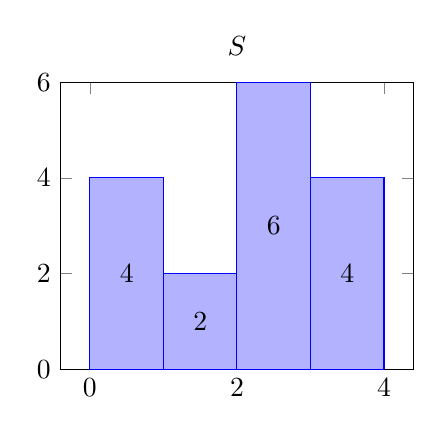
\begin{tikzpicture}
        \begin{axis}[
          width=0.5*\textwidth,
          title=$S$,
          ymin = 0,
          ymax=6,
          ]
          \addplot[
          ybar interval, 
          blue,fill=blue!30!white,
          ] plot coordinates
          {(0,4)(1,2)(2,6)(3,4)(4,4)};


    \node at (axis cs:0.5,2) {$4$};
    \node at (axis cs:1.5,1) {$2$};
    \node at (axis cs:2.5,3) {$6$};
    \node at (axis cs:3.5,2) {$4$};


     \end{axis}
      \end{tikzpicture}\qquad
     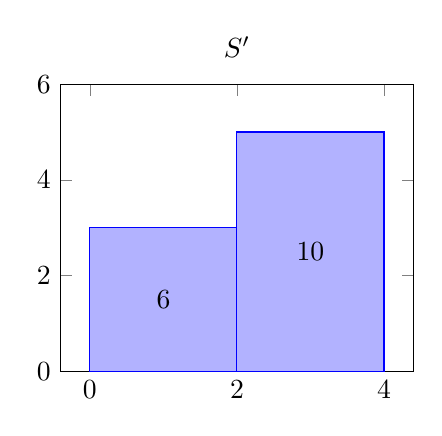
\begin{tikzpicture}
        \begin{axis}[
          width=0.5*\textwidth,
          title=$S'$,
          ymin = 0,
          ymax=6,
          ]

          \addplot[
          ybar interval, 
          blue,fill=blue!30!white,
          ] plot coordinates
          {(0,3)(2,5)(4,5)};

    \node at (axis cs:1,1.5) {$6$};
    \node at (axis cs:3,2.5) {$10$};


     \end{axis}
      \end{tikzpicture}


      \caption{Sèrie temporal amb àrea sota la corba i sèrie temporal
        resultant de la multiresolució amb agregació mitjana de la
        funció}
  \label{fig:multiresolucio:comptador}
\end{figure}






  \end{itemize}
  


La multiresolució, però, no pot conservar la resolució del comptatge,
així en l'exemple un cop s'ha consolidat $6=4+2$ no es pot tornar a
obtenir $4$ i $2$ llevat que es pogués reconstruir el senyal.  Com
s'ha exposat a
l'\autoref{ex:multireoslucio:informacio-subresolucions}, en consultes
en què l'interval no es correspongui amb les resolucions
emmagatzemades, els totals no seran els correctes que s'obtindrien de
calcular amb les dades originals.  De fet, és el mateix problema que
hem exposat que a partir d'un comptador no es poden deduir exactament
energies que no s'han mesurat.




% \todo{potser fer un exemple on es vegi com la multiresolució pot solucionar un problema d'inframostreig en els comptadors}




\subsection{Equivalències en l'agregació d'atributs}

Hi ha casos en què és el mateix aplicar una funció d'agregació
d'atributs que aplicar-ne una altra. En aquest apartat particularment
estudiem el cas de la $\glssymbol{not:sgstm:mitjanapd}$
(\seeref{def:sgstm:mitjanapd}) i el de la
$\glssymbol{not:sgstm:meanzohe}$ (\seeref{def:sgstm:meanzohe})
per a sèries temporals regulars.

Sigui $S=\{m_0,\dotsc,m_k\}$ una sèrie temporal
regular de període $p$ (\seeref{def:st:regular}) i sigui $[s,t]$
un interval de temps on $s=T(\min(S))-p=t_0-p$ i
$t=T(\max(S))=t_k$.  Demostrem que
$\glssymbol{not:sgstm:meanzohe}(S,[s,t]) =
\glssymbol{not:sgstm:mitjanapd}(S,[s,t])$ pel que fa al valor
resultant calculat negligint el temps resultant. És a dir en realitat demostrem
$V(\glssymbol{not:sgstm:meanzohe}(S,[s,t])) =
V(\glssymbol{not:sgstm:mitjanapd}(S,[s,t]))$ però no escrivim la
projecció de l'atribut de valor, $V()$, per a no complicar la notació.

La mitjana aritmètica de la sèrie temporal és
$\glssymbol{not:sgstm:mitjanapd}(S,[s,t])=\frac{v_0+\dotsb+v_k}{|S|}$.
%
La mitjana amb representació \gls{zohe} és
$\glssymbol{not:sgstm:meanzohe}(S,[s,t])= \frac{1}{t-s} (
v_0(t_0-s)+v_1(t_1-t_0)+\dotsb+ v_k(t_k-t_{k-1}) )$.

Per ser regular, $t_1-t_0 = \dotsb = t_k-t_{k-1} = p$. A més
$s=t_0-p$ i per tant $t_0-s = p$. També per ser regular, $t_k-t_0=
t_k +(- t_{k-1} + t_{k-1}) + \dotsb + (- t_1 + t_1) - t_0 = (|S|-1)p$
i per tant $t-s=t_k - (t_0 - p) = (|S|-1)d +p = |S|p$.

Reescrivint, $\glssymbol{not:sgstm:meanzohe}(S,[s,t])=
\frac{1}{|S|p} ( v_0p+v_1p+\dotsb+ v_kp ) = \frac{1}{|S|} (
v_0+v_1+\dotsb+ v_k ) = \glssymbol{not:sgstm:mitjanapd}(S,[s,t])$.



Així doncs, en una sèrie temporal regular es pot aplicar la
$\glssymbol{not:sgstm:mitjanapd}$ com a equivalent a la
$\glssymbol{not:sgstm:meanzohe}$; de fet la
\autoref{fig:multiresolucio:comptador} n'és un exemple. Un àmbit
d'aplicació d'aquestes equivalències pot ser el de simplificar els
càlculs en les consultes als \gls{SGSTM}, en els discs dels quals les
subsèries temporals normalment s'emmagatzemen regulars.
 








%%% Local Variables:
%%% TeX-master: "main"
%%% End:


%  LocalWords:  multiresolució
